\documentclass[12pt]{article}
\usepackage{fontspec}   %加這個就可以設定字體
\usepackage{xeCJK}       %讓中英文字體分開設置
\setmainfont{Times New Roman}
\setCJKmainfont{標楷體} %設定中文為系統上的字型,而英文不去更動,使用原TeX字型
\XeTeXlinebreaklocale "zh"             %這兩行一定要加,中文才能自動換行
\XeTeXlinebreakskip = 0pt plus 1pt     %這兩行一定要加,中文才能自動換行
\usepackage{amsmath, amsthm, amssymb} %引入數學符號的套件,例如實數R、定理Thm...
\usepackage{graphicx}                 %現在, 假設我們要插入 pic.png 這個圖檔, 使用
%\title{我是標題}
%\author{我是作者}
%\date{} %不要日期

\newcommand{\uA}       {\mbox{\boldmath$A$}}
\usepackage{textcomp}
\usepackage{array}
\usepackage{graphicx}
\usepackage{colortbl}
\usepackage{color,xcolor}
\usepackage{listings}
\usepackage{array,booktabs}   %這三個為表格使用的套件
\usepackage{textpos}
\usepackage{float}
\usepackage{listings}

\title{Statistical learning assignment 8- chapter 4}
\author{孫浩哲 \hspace{0.7cm} M072040002}
\date{November 8, 2018}
\begin{document}
\maketitle
\begin{itemize}
\item[7.]
\begin{align*}
p_{yes}(x)
&=\frac{\pi_{yes}\exp({-\frac{1}{2\sigma^2}}(x-10)^2)}{\pi_{yes}\exp({-\frac{1}{2\sigma^2}}(x-10)^2)+\pi_{no}\exp({-\frac{1}{2\sigma^2}}x^2)}\\
&=\frac{0.8\exp({-\frac{1}{72}}(x-10)^2)}{0.8\exp({-\frac{1}{72}}(x-10)^2)+0.2\exp({-\frac{1}{72}}x^2)}\\[4ex]
&\Rightarrow p_{yes}(4)\approx0.752
\end{align*}
Approximately\ $75.2\%$ that the company will issue a dividend.
\item[8.]
\ \\
The training error rate is close to\ $0$ if\ $K=1$, and average error rate is\ $18\%$, that means error rate of\ $36\%$ on the test data.So we prefer logistic regression.
\item[9.]
\ \\
(a.)
\begin{align*}
\frac{P(X)}{1-P(X)}=0.37\Rightarrow1.37P(X)=0.37,P(X)\approx0.27
\end{align*}
(b.)\\
$$P(X)=0.16$$
$$odds=\frac{P(X)}{1-P(X)}=\frac{0.16}{0.84}\approx0.19$$
\newpage
\item[12.]
(a)
\begin{verbatim}
> power=function()
+ {
+   result=2^3
+   print(result)
+ }
> power()
[1] 8
\end{verbatim}
(b)
\begin{verbatim}
> power2=function(x,a)
+ {
+   result=x^a
+   print(result)
+ }
> power2(3,8)
[1] 6561
\end{verbatim}
(c)
\begin{verbatim}
> power2(8,17)
[1] 2.2518e+15
\end{verbatim}
(d)
\begin{verbatim}
> power3=function(x,a)
+ {
+   result=x^a
+   return(result)
+ }
\end{verbatim}
\newpage
(e)\ \\
\raggedright{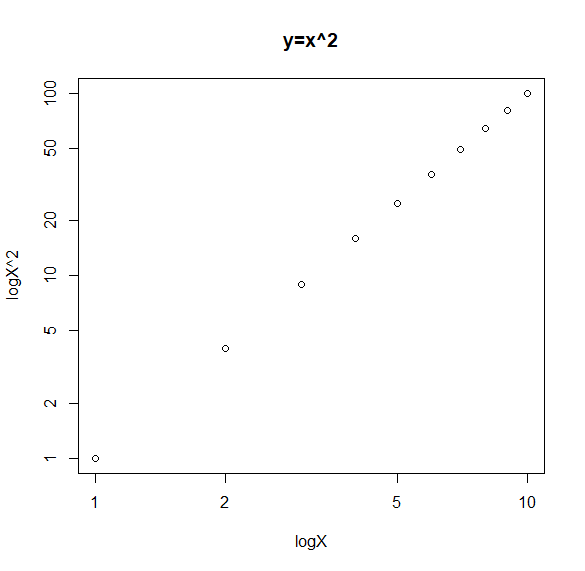
\includegraphics[width=0.6\linewidth]{x}}\\
(f)\ \\
\raggedright{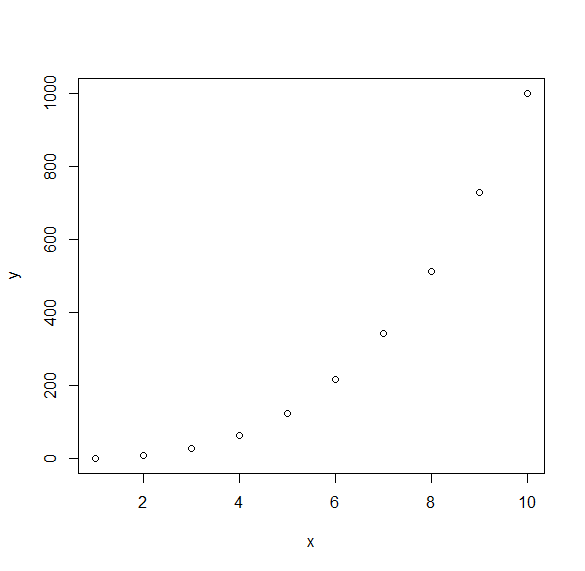
\includegraphics[width=0.6\linewidth]{3x}}
\item[13.]
\begin{verbatim}
> #######logistic regression#######
> {
+ class=rep(0,nrow(Boston))
+ class[which(crim>median(crim))]=1
+ boston=data.frame(Boston,class)
+ attach(boston)
+ model=glm(class~.-crim,data=boston,family=binomial)
+ tr=boston[1:400,]#training set
+ te=boston[401:506,]#test set
+ tecr=te$class#real test
+ pro=predict(model,data.frame(te),type="response")
+ tepre=rep(0,nrow(te))
+ tepre[which(pro>0.5)]=1
+ mean(tepre!=tecr)#test error
+ }
[1] 0.04716981
> #######LDA#######
> {
+ LD=lda(class~.-crim,data=boston,family=binomial)
+ telda=predict(LD,data.frame(te))
+ mean(telda$class!=tecr)
+ }
[1] 0.0754717
> #######KNN#######
> {
+ kn=knn(tr,te,tr$class,k=1)
+ mean(kn!=tecr)
+ }
[1] 0.0754717
> {
+ kn=knn(tr,te,tr$class,k=10)
+ mean(kn!=tecr)
+ }
[1] 0.0754717
> {
+ kn=knn(tr,te,tr$class,k=100)
+ mean(kn!=tecr)
+ }
[1] 0.09433962
\end{verbatim}
In this case we can find that the logistic regression is the best approach to predict, and the test error of LDA is equal to KNN when \ $K=1,10$.
\end{itemize}
\end{document} 